\documentclass[12pt,a4paper]{article}
\usepackage[utf8]{inputenc}
\usepackage[T1]{fontenc}
\usepackage[ngerman]{babel}
\usepackage{amsmath}
\usepackage{graphicx}
\usepackage{hyperref}
\usepackage[backend=biber,style=numeric]{biblatex}
\addbibresource{literatur.bib}

% Gleichungsnummerierung nach Abschnitt
\numberwithin{equation}{section}
% Abbildungsnummerierung nach Abschnitt
\usepackage{chngcntr}
\counterwithin{figure}{section}

% Benutzerdefinierte Referenznamen
\newcommand{\figref}[1]{Abb.~\ref{#1}}
\newcommand{\secref}[1]{Abschn.~\ref{#1}}

\begin{document}

\tableofcontents

\section{Einleitung}

Dies ist ein Verweis auf eine Gleichung~\eqref{eq:beispiel} und auf \figref{fig:beispielbild}.  
Ein Literaturverweis sieht so aus: \cite[][S.~2]{musterquelle}.  
Ein Abschnittsverweis: \secref{Details}.

\subsection{Hintergrund}
\subsubsection{Details}
\label{Details}
Dieser Abschnitt hat die Nummer 1.1.1

\section{Methoden}

\begin{equation}
    a^2 + b^2 = c^2
    \label{eq:beispiel}
\end{equation}

\begin{figure}[h]
    \centering
    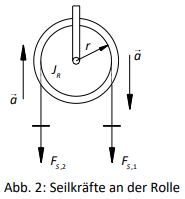
\includegraphics[width=0.4\textwidth]{beispielbild.png}
    \caption{Ein Beispielbild}
    \label{fig:beispielbild}
\end{figure}

abbildung:
    name: musterbild
    pfad: beispielbild.png
    caption: Ein Beispielbild
    label: beispielbild.png
    quelle:
        name: musterquelle
        seite: 2
    quelle: (eigene Darstellung)


\printbibliography

\end{document}
